\documentclass[12pt]{article}
\usepackage{natbib}
\usepackage[french]{babel}
\usepackage[T1]{fontenc}
\usepackage{url}
\usepackage[utf8x]{inputenc}
\usepackage{lastpage}
\usepackage{amsmath}
\usepackage{hyperref}
\usepackage{graphicx}
\usepackage{pdflscape}
\graphicspath{{images/}}
\usepackage{pdfpages}
\usepackage{parskip}
\usepackage{fancyhdr}
\usepackage{multicol}
\usepackage{vmargin}
\setmarginsrb{3 cm}{2.5 cm}{3 cm}{2.5 cm}{1 cm}{1.5 cm}{1 cm}{1.5 cm}

\title{ThermiScan}
\author{Lorenzo Bauduccio \\ Tom Ryser \\ Kevin Moreno}
\date{\today}

\makeatletter
\let\thetitle\@title
\let\theauthor\@author
\let\thedate\@date
\makeatother

\pagestyle{fancy}
\fancyhf{}
\rhead{Atelier Technicien 1\&2}
\lhead{Rapport - Arca'Box}
\cfoot{\thepage\ sur \pageref{LastPage}}
\rfoot{\footnotesize \thedate}

%$HeadURL: https://subversion.assembla.com/svn/cfpt-courses/trunk/_inc/inc_lst_csharp.tex $
%$LastChangedDate: 2016-10-12 16:29:50 +0200 (Wed, 12 Oct 2016) $
%$LastChangedRevision: 7006 $
%$LastChangedBy: marechal $

% lstlisting configuration for C#
%-------------------------------------------------------------------------------------
\usepackage{xcolor}
\usepackage{listings}
\usepackage{accsupp}

% color
\definecolor{lightgreen}{rgb}	{0.200, 0.980, 0.200}
\definecolor{darkgreen}{rgb}	{0.000, 0.400, 0.000}
\definecolor{lightgray}{gray}	{0.98}
\definecolor{darkred}{rgb}		{0.545, 0.000, 0.000}

% CSharp colors
\definecolor{class}{rgb}		{0.200, 0.600, 0.600}	% Cyan Visual Studio
\definecolor{keyword}{rgb}		{0.000, 0.000, 1.000}	% blue

% code to avoid line number copy during copy-paste from PDF
\newcommand{\noncopynumber}[1]{%
    \BeginAccSupp{method=escape,ActualText={}}%
    {\scriptsize#1}%
    \EndAccSupp{}%
}

% lstlisting parameters
\lstset {	
  language=[Sharp]C
, captionpos=b
, frame=shadowbox
, rulesepcolor=\color{gray}
% syntaxic coloration
, basicstyle=\footnotesize\ttfamily
, keywordstyle=\color{blue}
, commentstyle=\color{darkgreen}
, stringstyle=\color{darkred}
, backgroundcolor=\color{lightgray}
, identifierstyle=\color{black}
% lines numbering
, numbers=left
, numberstyle=\noncopynumber
, stepnumber=1
, numbersep=5pt
%
, breaklines=true
, tabsize=2
, showstringspaces=false
, lineskip={-1.5pt} % single line spacing
, escapeinside={/*(*@}{@*)*/}
, rangeprefix=//\{\  % slash, slash, curly left brace, space
, rangesuffix=\ \} % space, curly right brace
}

% Csharp : additional keywords
\lstset{
	morekeywords={var,get,set,string,value},
	otherkeywords={\#region,\#endregion,\#define,\#if,\#endif,\#else}, %morekeyword does not support # chararacter then we must use otherkeywords
	emph={[1]Application,
		Char,Color,Console,Convert,
		DialogResult,
		Environment,EventArgs,
		Form,
		Object,String,
		Assert,
		SByte,Int16,Int32,Int64,
		Byte,UInt16,UInt32,UInt64,
		Single,Double,
		Keys,KeyPressEventArgs,
		MessageBox,MessageBoxButtons},
	emphstyle={[1]\color{class}}
}

\lstset{prebreak=\raisebox{0ex}[0ex][0ex]
        {\ensuremath{\hookleftarrow}}}
%\lstset{postbreak=\raisebox{0ex}[0ex][0ex]
%        {\ensuremath{\hookrightarrow\space}}}
\lstset{breaklines=true, breakatwhitespace=true}

% replace sequence of char by another sequence of char
% see http://stackoverflow.com/questions/1116266/listings-in-latex-with-utf-8-or-at-least-german-umlauts
\lstset{literate=%
{ä}{{\"a}}1
{â}{{\^a}}1
{à}{{\`a}}1
{Ä}{{\"A}}1
{Â}{{\^A}}1
{À}{{\`A}}1
{ë}{{\"e}}1
{ê}{{\^e}}1
{é}{{\'e}}1
{è}{{\`e}}1
{Ë}{{\"E}}1
{Ê}{{\^E}}1
{É}{{\'E}}1
{È}{{\`E}}1
{ï}{{\"i}}1
{î}{{\^i}}1
{Ï}{{\"I}}1
{Î}{{\^I}}1
{ö}{{\"o}}1
{ô}{{\^o}}1
{Ö}{{\"O}}1
{Ô}{{\^O}}1
{ü}{{\"u}}1
{û}{{\^u}}1
{ù}{{\`u}}1
{Ü}{{\"U}}1
{Û}{{\^U}}1
{Ù}{{\`U}}1
{ç}{{\c c}}1
{Ç}{{\c C}}1
{°}{{\textsuperscript{o}}}1
% suppress BOM (Byte Order Mark) characters at the beginning of Visual Studio source
% see http://tex.stackexchange.com/questions/5935/how-to-suppress-bom-effect-in-the-output
{ï}{}0
{»}{}0
{¿}{}0
}


\begin{document}

%%%%%%%%%%%%%%%%%%%%%%%%%%%%%%%%%%%%%%%%%%%%%%%%%%%%%%%%%%%%%%%%%%%%%%%%%%%%%%%%%%%%%%%%%

\begin{titlepage}
	\centering
    
\includegraphics[scale = 1]{logo-cfpt-site.png}\\[1.5 cm]
    \textsc{\LARGE CFPT Informatique}\\[2.0 cm]
	\textsc{\Large Atelier Techniciens 1\&2 - Rapport}\\[0.5 cm]
	\rule{\linewidth}{0.2 mm} \\[0.4 cm]
	{ \huge \bfseries \thetitle}\\
	\rule{\linewidth}{0.2 mm} \\[1.5 cm]
	
	\begin{minipage}{0.4\textwidth}
		\begin{flushleft} \large
			\emph{Étudiants:}\\
			\theauthor
			\end{flushleft}
			\end{minipage}~
			\begin{minipage}{0.4\textwidth}
			\begin{flushright} \large
			\emph{Enseignant:} \\
			Francisco Garcia
		\end{flushright}
	\end{minipage}\\[2 cm]
	
	{\large \thedate}\\[0.5 cm]
 
	\vfill
	
\end{titlepage}

%%%%%%%%%%%%%%%%%%%%%%%%%%%%%%%%%%%%%%%%%%%%%%%%%%%%%%%%%%%%%%%%%%%%%%%%%%%%%%%%%%%%%%%%%

\setcounter{page}{2}
\tableofcontents
\pagebreak

%%%%%%%%%%%%%%%%%%%%%%%%%%%%%%%%%%%%%%%%%%%%%%%%%%%%%%%%%%%%%%%%%%%%%%%%%%%%%%%%%%%%%%%%%

\section{Cahier des charges}
\subsection{Description du projet}
Nous devons réaliser une application en Web qui doit nous permettre d’afficher une vidéo venant du smartphone CAT S60, qui possède une caméra thermique. L’application Web doit permettre de gérer plusieurs vidéos venant de plusieurs caméras, et permettre d’afficher une courbe de température.
\subsection{Travail à réaliser}
\begin{itemize}
    \item Réaliser une application en Web qui s'approche un maximum d'un point de vue fonctionnel de l'application FLIR Tools Mobile.
    \begin{itemize}
        \item Affichage d’un graphique montrant la température maximal, minimal et la moyenne.
        \item Affichage de la vidéo.
        \item Gestion de plusieurs vidéos venant d’une seule caméra. 
    \end{itemize}
\end{itemize}
\subsection{Outils utilisés}
\begin{itemize}
     \item Visual Studio Code
     \item EasyPHP V 14.1
     \item MySQL
     \item Python 3
     \item Balsamiq Mockups 3
\end{itemize}

\subsection{Comment avons-nous procédé ?}
\begin{itemize}
     \item Réalisation d’une maquette du front-end
     \item Création d’un exécutable à partir d’un programme python
     \item Création d’une base de données pour les utilisateurs, les caméras et les vidéos
     \item Réalisation du front-end avec easyPHP
     \item Ajout d’un script JS permettant d’afficher un graphique
     \item Mise au propre du code
\end{itemize}

\clearpage

\section{Réalisations}
\subsection{Application de sélection des jeux}
L'application permettant de sélectionner  les jeux à été réalisé avec Unity 3D, nous avons utilisé l'asset gratuite \textit{SliderMenu} que nous avons un peu modifié pour quel corresponde à nos exigences.

\subsubsection{Ajout de jeux}
Pour ajouter un jeu sur l'application, il suffit d'ajouter un dossier nommé par le nom du jeu et contenant les dossiers respectant la hiérarchie suivante :
\begin{itemize}
    \item App
    \begin{itemize}
        \item \textit{Contient les fichiers du jeu}
        \item \textbf{game.exe} (L'exécutable du jeu doit être nommer comme-ça)
    \end{itemize}
    \item image.jpg
\end{itemize}
\subsubsection{Lancement automatique}
Pour pouvoir lancer automatiquement l'application de sélection de jeux, il suffit de placer un raccourci de l'exécutable de l'application dans le dossier de démarrage automatique d'application accessible en effectuant la commande \texttt{shell:startup} sur la boite de dialogue \texttt{Éxecuter (Win + R)}.

\clearpage

\subsubsection{Login automatique à une session}
Tout d'abord, il faut se rendre sur la boite de dialogue \texttt{Éxecuter (Win + R)} et entrer la commande suivante : \texttt{control userpasswords2}

\begin{figure}[htp]
    \centering
    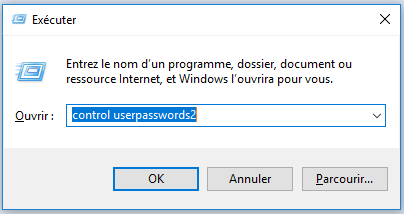
\includegraphics[scale=.75]{control_passwords.png}
    \caption{Commande d'accès aux contrôle des mots de passes}
    \label{fig:control_passwords}
\end{figure}

Ensuite, il faut cliquer sur l'utilisateur que l'on veut déconnecter automatiquement et décocher la case \textit{Les utilisateurs doivent entrer un nom d'utilisateur et un mot de passe pour utiliser cet ordinateur}.

\begin{figure}[h]
    \centering
    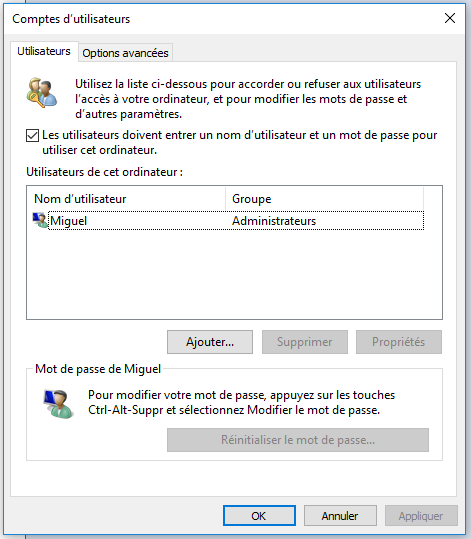
\includegraphics[scale=.6]{users.png}
    \caption{Dés-activation du mot de passe pour un compte utilisateur}
    \label{fig:users}
\end{figure}

Il suffira ensuite de confirmer le retrait du mot de passe pour le compte pour lui permettre de se connecter automatiquement.

\clearpage

\begin{figure}[h]
    \centering
    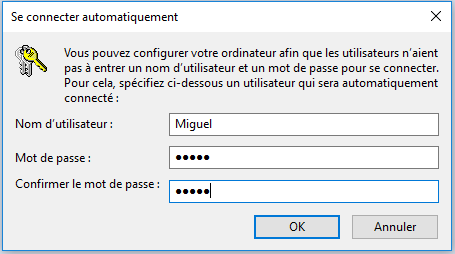
\includegraphics[scale=.6]{confirm_session.png}
    \caption{Confirmation du passage en mode connexion automatique}
    \label{fig:confirm_password}
\end{figure}

\subsubsection{Description du code}
Le code gérant les jeux se trouve dans \texttt{GameLoader.cs}, d'abord la fonction \texttt{Start} (appelé lors de l'initialisation de la classe). Elle initialise le dictionnaire de jeux, récupère la liste de slides se trouvant sur la classe \texttt{SliderMenu} se trouvant sur la caméra principale, on désactive la visibilité du curseur et on charge la liste des jeux.
\begin{lstlisting}
void Start()
{
    this.Games = new Dictionary<string, string>();

    GameObject camera = GameObject.Find("Main Camera");
    SliderMenu script = camera.GetComponent<SliderMenu>();
    Slides = script.Slides = new List<GameObject>();

    Cursor.visible = false;

    LoadGames();
}
\end{lstlisting}

La fonction \texttt{Update} est appelée à chaque \textit{frame}, dans cette fonction, on vérifie les boutons appuyiez par les joueurs et on effectue une action approprié pour chaque entré clavier. Lors de l'utilisation des joysticks vers la gauche ou la droite on invoque les cliques des boutons permettant de changer de slide. Lors de l'appui sur le bouton \textit{8 (Dollars)}, on coupe le volume de la musique du menu puis récupérons le nom du jeu puis un \textit{Process} va lancer l'exécutable du jeu sélectionner.
\begin{lstlisting}
void Update()
{
    if (Input.GetKeyDown(KeyCode.LeftArrow) || Input.GetKeyDown(KeyCode.A))
    {
        btnLeft.onClick.Invoke();
    }

    if (Input.GetKeyDown(KeyCode.RightArrow) || Input.GetKeyDown(KeyCode.D))
    {
        btnRight.onClick.Invoke();
    }

    if (Input.GetKeyDown(KeyCode.Alpha8))
    {
        audioSource.volume = 0f;

        string selectedGame = slides.transform.GetChild(slides.transform.childCount - 1).name;

        UnityEngine.Debug.Log(audioSource.volume);

        string path = @"" + Games[selectedGame] + "\\App\\game.exe";

        Process gameApp = new Process();
        gameApp.StartInfo.FileName = path;
        gameApp.Start();
    }
}
\end{lstlisting}

La fonction \texttt{OnApplicationFocus} est appelée lorsque le menu à de nouveau le \textit{focus}, alors on remet le volume sonore de la musique au maximum.
\begin{lstlisting}
void OnApplicationFocus(bool hasFocus)
{
    if (hasFocus)
        audioSource.volume = 100f;
}
\end{lstlisting}

La fonction \texttt{OnApplicationFocus} va charger la liste des jeux, créer les objets nécessaire pour être ajouté à l'objet \textit{Slider} avec toutes les données nécessaire : nom, texte, image.
\begin{lstlisting}
private void LoadGames()
{
    DirectoryInfo dir = new DirectoryInfo(GAME_DIRECTORY);

    foreach (DirectoryInfo d in dir.GetDirectories())
    {
        this.Games.Add(d.Name, d.FullName);
    }

    foreach (var game in this.Games)
    {

        GameObject gmObj = Instantiate(gameExample, transform.position, transform.rotation);
        Text gmObjText = gmObj.GetComponentInChildren<Text>();
        Image gmObjImage = gmObj.GetComponentInChildren<Image>();
        
        //Load values
        gmObj.transform.SetParent(slides.transform);
        gmObj.name = game.Key;
        gmObjText.text = game.Key;

        //Load image
        byte[] data = File.ReadAllBytes(game.Value + "\\image.jpg");
        Texture2D texture = new Texture2D(64, 64, TextureFormat.ARGB32, false);
        texture.LoadImage(data);
        gmObjImage.sprite = Sprite.Create(texture, new Rect(0.0f, 0.0f, texture.width, texture.height), new Vector2(0.5f, 0.5f), 100f);

        Slides.Add(gmObj);
    }
}
\end{lstlisting}

\section{Conclusion}
\subsection{Bilan}
Dans l’ensemble, nous sommes plutôt satisfaits de notre projet. Nous avons atteint les buts les plus importants.
\subsection{Problèmes rencontrés}
\subsubsection{Téléphone ne permettant pas la diffusion en direct}
Le problème majeur rencontré dès le début du projet est l’indisponibilité de live streaming du Cat S60. Selon les pages qu’on parcourait, il était mentionné que la Cat S60 possédait une option de live streaming, ce qui n’est au final pas le cas, contrairement à la nouvelle génération du Cat, le S61. Étant donné que le cahier des charges était de faire un live directement via une application web, nous nous sommes retrouvé à devoir modifier le cahier des charges, qui est passé d’un live sur une application web à juste afficher une vidéo.
\subsubsection{Affichage d'un graphique}
Plusieurs problèmes se sont joint lors de la création du graphique. Premièrement, il nous fallait trouver un script JS permettant d’afficher un graphique à partir de valeur venant d’un fichier CSV. Lors de nos premiers tests, le problème principal était l’importation de nos valeurs dans les tableaux, les graphiques ne possédant pas de tableau souple au niveaux des données entrées. Nous avons essayé avec un graphique venant de \url{www.amcharts.com} et un autre venant de \url{www.highcharts.com}. En fin de compte, Nous nous sommes occupé d’en faire un, en reprenant des parties de code provenant des anciens tests. 

\clearpage

\addcontentsline{toc}{section}{\listfigurename}
\listoffigures

\end{document}
